\documentclass[11pt]{article}

\usepackage{authblk}
\usepackage[a4paper,margin=1.8cm]{geometry}
\usepackage[utf8]{inputenc}
\usepackage{mathptmx} % times roman, including math
\usepackage[hyphens]{url}
\usepackage{doi}
\usepackage{hyperref}
\usepackage[numbers,sort]{natbib}
\usepackage{amsmath}
\usepackage{amssymb}
\usepackage{amsthm}
\usepackage{stmaryrd} % \llbracket etc.
\usepackage{algorithm}
\usepackage{algpseudocode} % layout for algorithmicx package, provides "algorithmic" environment for pseudocode
\usepackage{setspace}
\usepackage{csquotes}
\usepackage{tikz}
\usepackage{mdwlist}

\usetikzlibrary{arrows.meta}
\hyphenation{da-ta-cen-ter da-ta-cen-ters time-stamp time-stamps time-stamped Grish-chen-ko}
\frenchspacing

\usepackage{isabelle,isabellesym}
\isabellestyle{it}

\newtheorem{proposition}{Proposition}

\begin{document}
\sloppy
\title{OpSets: Sequential Specifications for Replicated Datatypes}
\author[1]{Martin Kleppmann\thanks{Corresponding author. Email: martin.kleppmann@cl.cam.ac.uk}}
\author[1]{Victor B.\ F.\ Gomes}
\author[2]{Dominic P.\ Mulligan}
\author[1]{Alastair R.\ Beresford}
\date{}

\affil[1]{Department of Computer Science and Technology, University of Cambridge, UK}
\affil[2]{Security Research Group, Arm Research, Cambridge, UK}

\maketitle

\begin{center}
Regular Paper
\end{center}

\begin{abstract}
We introduce OpSets, a framework for specifying and reasoning about the semantics of replicated datatypes that provide eventual consistency in a distributed system, and formally verifying algorithms that implement these datatypes.
Our approach is simple but expressive, allowing us to succinctly specify a variety of abstract datatypes, including maps, sets, lists, text, graphs, trees, and registers.
Our datatypes are also composable, enabling the construction of complex data structures.
To demonstrate the utility of OpSets for analysing replication algorithms, we highlight an important correctness property for collaborative text editing that has traditionally been overlooked; algorithms that do not satisfy this property can exhibit awkward interleaving of text.
We use OpSets to specify this correctness property and prove that although one existing replication algorithm satisfies this property, several other published algorithms do not.
We also show how OpSets can be used to develop new replicated datatypes: we provide a simple specification of an atomic move operation for trees, an operation that had previously been thought to be impossible to implement without locking.
We use the Isabelle/HOL proof assistant throughout to formalise the OpSets approach and produce mechanised proofs of correctness of the main claims in this paper, thereby eliminating the ambiguity of previous informal approaches, and ruling out reasoning errors that could occur in handwritten proofs.
\end{abstract}
\clearpage

\section{Introduction}

A common requirement across many distributed systems is that several nodes may concurrently access and manipulate some shared data structure.
Examples include everything from journalists using their laptops to work on a shared text document to a set of front-end web-servers manipulating a common database.
In doing so, it is important that the shared data satisfies certain \emph{consistency guarantees}.
For example, strong consistency models such as serializability \cite{Kleppmann:2017wj} or linearizability \cite{Herlihy:1990jq} make a system behave like a single sequentially executing node, even when it is in fact replicated and concurrent.
An unavoidable downside of these models is that any operation or transaction must wait for network communication before it is allowed to complete \cite{Davidson:1985hv,Gilbert:2002il}.
Thus, in a system with strong consistency, a node cannot make progress while it is offline or partitioned from other nodes.

On the other hand, \emph{eventual consistency} \cite{Bailis:2013jc,Burckhardt:2014hy,Terry:1994fp,Vogels:2009ca} allows each participant to modify a local copy (\emph{replica}) of a shared data structure while offline, but its definition is very weak: \emph{``if no new updates are made to the shared state, all nodes will eventually have the same data.''}
The premise \emph{if no new updates are made} may never be true if the shared state is continually modified because the system is never quiescent.
Moreover, the final system state is unconstrained: nothing in the definition of eventual consistency specifies which states are legal.

Conflict-free Replicated Data Types, or CRDTs \cite{Shapiro:2011wy,Shapiro:2011un}, are abstractions for replicated state that have received significant attention in recent years (see \S~\ref{sec:relwork}).
The primary correctness property for CRDTs is \emph{convergence} \cite{Shapiro:2011un,Gomes:2017gy}, defined as: \emph{``whenever any two replicas have applied the same set of updates, they are in the same state''}, even if each replica applies the updates in a different order.
Convergence is a stronger property than eventual consistency, but it also fails to define what the converged state should be.

In this work we introduce \emph{Operation Sets} (or \emph{OpSets} for short), a novel approach for specifying the semantics of replicated datatypes, and reasoning about algorithms for concurrent data access and manipulation.
We go beyond merely ensuring replica convergence: the OpSets approach is a form of executable specification that precisely defines the permitted states of a replica after some set of updates has been applied.
Our contributions in this paper are as follows:

\begin{itemize*}
\item In \S~\ref{sec:approach} we introduce the OpSet, a new abstraction for specifying and reasoning about the consistency properties of concurrently editable data structures.

\item On top of this abstraction, in \S~\ref{sec:datatypes} and \S~\ref{sec:tree}, we specify a variety of composable abstract datatypes (maps, sets, lists, text, graphs, trees, and registers), and we argue that our specifications are both simple and precise, making them a suitable tool for reasoning about replicated data.

\item In \S~\ref{sec:bad-merge} we demonstrate how the OpSet abstraction can be used to reason about existing algorithms. We highlight an important correctness property for collaborative text editing that has been overlooked by prior work in this area.
Our specification is, to our knowledge, the first that correctly captures this property.
We then review a selection of text editing CRDTs from the literature, prove that one satisfies our specification, and identify several others that fail to satisfy our correctness property.

\item In \S~\ref{sec:tree} we show how the OpSet abstraction can be used to develop new replicated datatypes. In particular we describe, for the first time, how an atomic move operation can be defined for a tree CRDT.
This operation can be used to move a subtree to a new position within the tree, or to rename a key in a map, or to reorder items in a list.
The OpSets approach enables a simple definition of this operation that had previously been thought impossible without locking \cite{Najafzadeh:2017vk}.

\item Using the Isabelle/HOL proof assistant~\cite{DBLP:conf/tphol/WenzelPN08} we formalise the OpSets approach, producing mechanised proofs of correctness of the main claims in this paper.
In particular, we prove that our list specification is strictly stronger than the recent specification of collaborative text editing by Attiya et al. \cite{Attiya:2016kh}.
By using mechanised proofs we eliminate the ambiguity of previous informal approaches, and rule out reasoning errors that could occur in handwritten proofs.
\end{itemize*}

\section{The OpSets Approach}\label{sec:approach}

The OpSets approach is a simple abstraction for describing the consistency properties of a replicated data system.
We outline the general approach in this section, before describing concrete data structures and specifications in \S~\ref{sec:datatypes} and \S~\ref{sec:tree}.

\subsection{System Model}\label{sec:system-model}

We assume that the system consists of a set of \emph{nodes} connected by a \emph{network}.
These nodes concurrently access some \emph{shared data structure}, which may be a relational database (consisting of rows in tables), a text document (a sequence of characters), a vector-graphics document (a tree of records describing graphical objects), a filesystem (a tree of directories and files), or any other kind of data structure.

New nodes can be added at any time, and the set of nodes need not be known in advance.
Nodes might be mobile devices, and hence we assume that nodes are sometimes \emph{offline}, i.e.\ temporarily unable to communicate with other nodes.
We require that nodes can access the shared data anytime, even while offline.
Thus, each node has a local copy of the shared data structure, which it can read and modify without waiting for any communication or coordination with other nodes.

Whenever a node makes a modification to that structure, it records the change as an \emph{operation}.
For example, an operation may describe an insertion at a particular position in a text document.
Each node locally maintains a set of operations, the \emph{OpSet}.
Whenever a node makes a change to the shared data, it adds the corresponding operation to its OpSet, and also sends \emph{messages} containing the operation to other nodes.
Whenever a node receives a message from another node, the operation in that message is added to the recipient's local OpSet.
Operations remain immutable throughout this process.

We make no assumptions about the reliability of the network: messages may be lost, duplicated, or arbitrarily reordered.
Reflecting the characteristics of real networks, we assume that lost messages are retransmitted when possible (e.g.\ using TCP), but messages may be permanently lost due to network or node failures.
Since the OpSet at each node is a monotonically growing set of operations, any two communicating nodes can merge their OpSets using the standard set union operator $\cup$.
Set union is commutative, associative, and idempotent, ensuring that communicating nodes converge towards the same OpSet contents.

We assume that each operation has a unique identifier (ID), that new IDs can be generated by any node without communication with other nodes, and that we have a total ordering on operation IDs.
These requirements can easily be met by using Lamport timestamps \cite{Lamport:1978jq} as IDs.
A Lamport timestamp is a pair $(\mathit{counter}, \mathit{nodeID})$ that is constructed as follows:
\begin{itemize}
\item $\mathit{counter}$ is an integer.
    To generate a new ID, find the maximum counter of any existing operation ID in the local OpSet, and increment that number.
\item $\mathit{nodeID}$ is a string that uniquely identifies the node generating the ID, e.g.\ a UUID \cite{Leach:2005hm}.
\end{itemize}

Although different nodes may generate IDs with the same counter value, each node generates IDs with strictly increasing counter values, and thus IDs are globally unique.
We define the total order on IDs as being the lexicographic order:
\[
    \,(\mathit{ctr}_1, \mathit{node}_1) < (\mathit{ctr}_2, \mathit{node}_2)\,
    \;\Longleftrightarrow\;
    \mathit{ctr}_1 < \mathit{ctr}_2 \;\vee\;
    (\mathit{ctr}_1 = \mathit{ctr}_2 \wedge \mathit{node}_1 <\mathit{node}_2).
\]

%This total order is a linear extension of the partial order that captures their causal dependencies (the \emph{happens-before} relation).
%That is, whenever a node changes the shared data and generates a new operation, the ID of the new operation must be strictly greater than that of any existing operation in the OpSet of the node generating the new operation.

\subsection{Interpreting an OpSet}\label{sec:op-serial}

Most definitions of operation-based CRDTs describe how a node's local state is manipulated by operations \cite{Shapiro:2011wy,Shapiro:2011un}.
We now depart from this convention and present an alternative formulation of replicated datatypes.

In the OpSets approach, we require that the shared data structure is never manipulated directly.
Instead, we use an \emph{interpretation function} $\llbracket-\rrbracket$ that takes an OpSet $O$ and returns the current state $\llbracket O \rrbracket$ of the shared data structure described by the OpSet.
The interpretation function is \emph{pure}, i.e.\ deterministic, side-effect free, and its result depends only on $O$.
All nodes in the system employ the same interpretation function.

Consequently, whenever any two nodes have the same OpSet $O$, their view of the shared data structure $\llbracket O \rrbracket$ must also be equal.
This construction trivially ensures eventual consistency: as two nodes converge towards the same OpSet contents, any data structure that is deterministically derived from the OpSet must also converge.

In principle, any deterministic function can serve as interpretation function.
However, in defining the semantics of CRDTs (see \S~\ref{sec:datatypes} and \S~\ref{sec:tree}), we have found it useful to specialise $\llbracket-\rrbracket$ such that we can interpret one operation at a time.

Let the OpSet $O$ be a set of pairs $(\mathit{id},\, \mathit{op})$, where $\mathit{id}$ is a unique operation identifier and $\mathit{op}$ is an arbitrary description of the change that occurred.
Assume that we have a total ordering $<$ on identifiers, as explained in \S~\ref{sec:system-model}.
Then observe that for any OpSet there exists a unique sequence of operations, containing all operations of the OpSet in ascending order of their identifier.
We can specify the semantics of each operation~--- that is, the effect of the operation on the OpSet interpretation~--- when applied in this sequential order.

Formally, we can define the interpretation $\llbracket O \rrbracket$ of the OpSet $O$ as follows:
\begin{align*}
    \big\llbracket \emptyset \big\rrbracket &= \mathsf{InitialState} \\
    \big\llbracket O \;\cup\; \{(\mathit{id},\, \mathit{op})\} \big\rrbracket &=
    \mathsf{interp}\big[\llbracket O \rrbracket,\, (\mathit{id},\, \mathit{op})\big]
    \qquad\text{ provided that } \forall\,(\mathit{id}',\, \mathit{op}') \in O.\; \mathit{id}' < \mathit{id}
\end{align*}
where $\mathsf{interp}\big[S,\, (\mathit{id},\, \mathit{op})\big]$ is the interpretation of the operation $(\mathit{id},\, \mathit{op})$ in the state $S$, and $\mathsf{InitialState}$ is a fixed minimal element (e.g. the empty tree, or empty list) of the replicated type described.
In other words, if $S$ is the result of interpreting all operations with identifiers less than $\mathit{id}$, then
$\mathsf{interp}\big[S,\, (\mathit{id},\, \mathit{op})\big]$ is the interpretation of the OpSet to which $(\mathit{id},\, \mathit{op})$ has been added.
For example, if $\mathit{id}_1 < \mathit{id}_2 < \mathit{id}_3$, we have:
\begin{align*}
    \big\llbracket \{(\mathit{id}_1,\ \mathit{op}_1),\;
    &(\mathit{id}_2,\ \mathit{op}_2),\,
    (\mathit{id}_3,\ \mathit{op}_3)\} \big\rrbracket \;=\\
    &\mathsf{interp}\big[\mathsf{interp}\big[\mathsf{interp}\big[\mathsf{InitialState},\,
    (\mathit{id}_1,\ \mathit{op}_1)\big],\,
    (\mathit{id}_2,\ \mathit{op}_2)\big],\,
    (\mathit{id}_3,\ \mathit{op}_3)\big]
\end{align*}
Provided that the operation interpretation $\mathsf{interp}\big[S,\, (\mathit{id},\, \mathit{op})\big]$ is deterministic, the OpSet interpretation function $\llbracket-\rrbracket$ is also deterministic, due to the fact that the operation order in the OpSet is unique.

\subsection{Receiving Messages Out-of-order}\label{sec:order-change}

Many computing systems are based on the idea of putting operations in some total order, and executing them in that order.
For example, serializable transactions \cite{Kleppmann:2017wj} and state machine replication \cite{Schneider:1990vy} follow this approach.
However, it is important to understand that the OpSet interpretation of \S~\ref{sec:op-serial} relies on a weaker notion of ordering than most systems.

With serializable transactions and state machine replication, once a transaction/operation has been executed in some state, its results are expected to be durable.
Thus, before executing some transaction $T_i$, the system needs to ensure that there is no pending transaction with a lower ID than $T_i$ (which would need to be executed before $T_i$), since otherwise the subsequent arrival of a transaction with lower ID would invalidate the state in which $T_i$ was executed.
However, ensuring this precondition is expensive: as we show in \S~\ref{sec:op-sequences}, it requires communication with at least a quorum of nodes; if the IDs are Lamport timestamps, it even requires communication with every single node \cite{Lamport:1978jq}.
If too many nodes are offline, the system cannot execute any transactions.

By contrast, our system model of \S~\ref{sec:system-model} requires nodes to always be able to read and modify the shared data, even when all nodes are offline.
Moreover, we do not assume any ordering guarantees from the network.
Thus, whenever there is some operation $(\mathit{id}_1, \mathit{op}_1) \in O$ in the OpSet $O$ of some node, it is possible that the node will subsequently receive a message containing $(\mathit{id}_2, \mathit{op}_2)$, where $\mathit{id}_2 < \mathit{id}_1$; that is, the later-arriving operation needs to be applied before the existing operation $(\mathit{id}_1, \mathit{op}_1)$ in the OpSet interpretation $\llbracket O \rrbracket$.

In the OpSet model, such out-of-order delivery of operations is no problem: the order in which operations are received has no effect on the OpSet $O$, and since we assume the interpretation function to be pure and side-effect free, the interpretation $\llbracket O \rrbracket$ can always be recomputed whenever new operations are added to $O$.

The interpretation function is an \emph{executable specification} that defines the expected result of interpreting a set of operations.
Presenting replicated datatypes in this manner has two significant advantages:
\begin{enumerate*}
\item
Unlike typical definitions of CRDT algorithms \cite{Shapiro:2011wy,Shapiro:2011un}, it is not necessary for the interpretation function $\mathsf{interp}\big[S,\, (\mathit{id},\, \mathit{op})\big]$ to commute with respect to other operations: any pure function can be used.
This fact makes it much simpler to specify the interpretation of operations, as we shall see in \S~\ref{sec:datatypes} and \S~\ref{sec:tree}.
\item
We can guarantee the existence of an implementation of each described datatype: the specification itself.
This is in contrast to axiomatic specifications, which may not be implementable, and require additional work to demonstrate than an implementation exists which satisfies the axiomatic description.
\end{enumerate*}

For practical implementations of replicated datatypes, a naive OpSet interpretation may exhibit poor performance, since nodes must potentially apply the same subset of operations repeatedly.
More efficient (and, most likely, more complex) algorithms for CRDTs can therefore be developed and shown to satisfy the OpSet-based specification---we do this in \S~\ref{sec:bad-merge}.

However, we have developed a practical JavaScript CRDT implementation around the OpSet model,\footnote{\url{https://github.com/automerge/automerge}} and found it to have some advantages: for example, users can easily inspect the editing history of a document, since every past version of the document is the interpretation of a particular subset of operations.
Moreover, using OpSets provides a straightforward mechanism for recovering from network partitions and failures, as missing operations may be retransmitted and added to the OpSets of previously partitioned nodes.
The details of this implementation are beyond the scope of this paper.

\section{Specifying a Graph of Lists, Maps, and Registers}\label{sec:datatypes}

We now make the OpSets approach concrete by defining example semantics for commonly-used data structures: maps (which associate values with user-specified keys) and lists (linear sequences of values).
The map datatype can also represent a set (by using keys as members of the set, and ignoring values).
The list datatype can also represent text (by mapping each character to a list element).
In both lists and maps the values may be primitives (such as numbers or strings), or references to other map or list objects.
Using these references we can construct arbitrary object graphs, including cycles of object references, like in object-oriented programming languages.
In Section~\ref{sec:tree} we will show how to restrict this object graph so that it conforms to a tree structure.

We treat each key of a map, and each element of a list, as a multi-value register.
That is, if there are several concurrent assignments to the same map key or list element, our datatype preserves all concurrently written values.
Thus, reading a map key or list element may return multiple values, which may be merged explicitly by the user.
Assigning a new value to a map key or list elements overwrites all causally preceding values.
Different register behaviour, such as last-writer-wins (arbitrarily picking one of the concurrently written values as winner), can easily be defined, as we show later.

\subsection{Generating Operations}\label{sec:datatypes-gen}

An OpSet for these datatypes may contain six types of operation:
\begin{description}
    \item[$(\mathit{id},\, \mathsf{MakeMap})$] creates a new, empty map object.
        $\mathit{id}$ may henceforth be used to identify this object.
    \item[$(\mathit{id},\, \mathsf{MakeList})$] creates a new, empty list object.
        $\mathit{id}$ may henceforth be used to identify this object.
    \item[$(\mathit{id},\, \mathsf{MakeVal}(\mathit{val}))$] associates the ID $\mathit{id}$ with the primitive value $\mathit{val}$ (e.g.\ a number, string, or boolean).
        This operation is used to ``wrap'' any primitive value, allowing $\mathsf{Assign}$ operations (see below) to always use IDs as values, regardless of whether the value is a primitive value, or a reference to a map or list object.
    \item[$(\mathit{id},\, \mathsf{InsertAfter}(\mathit{ref}))$] creates a new list element with ID $\mathit{id}$, and inserts it into a list.
        If $\mathit{ref}$ is the ID of a prior $\mathsf{MakeList}$ operation, then the new element is inserted at the head of that list.
        Otherwise $\mathit{ref}$ must be the ID of an existing list element (i.e.\ a prior $\mathsf{InsertAfter}$ operation), in which case the new list element is inserted immediately after the referenced list element.
        Note that the $\mathsf{InsertAfter}$ operation does not associate a value with the new list element; that is done by a subsequent $\mathsf{Assign}$ operation.
    \item[$(\mathit{id},\, \mathsf{Assign}(\mathit{obj}, \mathit{key}, \mathit{val}, \mathit{prev}))$] assigns a new value to a key within a map (if $\mathit{obj}$ is the ID of a prior $\mathsf{MakeMap}$ operation), or to a list element (if $\mathit{obj}$ is the ID of a prior $\mathsf{MakeList}$ operation).
        In the case of map assignment, $\mathit{key}$ is the user-specified key to be updated, which may be any primitive value such as a string or integer.
        In the case of a list, $\mathit{key}$ is the ID of the list element to be updated (i.e.\ the ID of a prior $\mathsf{InsertAfter}$ operation).
        $\mathit{val}$ is the ID of the value being assigned, which may identify a $\mathsf{MakeMap}$, $\mathsf{MakeList}$, or $\mathsf{MakeVal}$ operation.
        $\mathit{prev}$ is the set of IDs of prior $\mathsf{Assign}$ operations to the same key in the same object, which are overwritten by the present operation.
    \item[$(\mathit{id},\, \mathsf{Remove}(\mathit{obj}, \mathit{key}, \mathit{prev}))$] removes a key-value pair from a map, or an element from a list.
        As with $\mathsf{Assign}$, $\mathit{obj}$ is the ID of the prior $\mathsf{MakeMap}$ or $\mathsf{MakeList}$ operation that created the object being updated, and $\mathit{key}$ identifies the key or list element being removed.
        $\mathit{prev}$ is the set of IDs of prior $\mathsf{Assign}$ operations to the same key in the same object, which are removed by the present operation.
\end{description}

\floatname{algorithm}{Listing}
\begin{algorithm}[t]
\caption{Generating new operations for modifying maps and lists.}\label{fig:pseudocode}
\noindent
\renewcommand\algorithmicindent{10pt}
\begin{minipage}[t]{0.5\textwidth}
\begin{algorithmic}
    \Function{setMapKey}{$O, \mathit{map}, \mathit{key}, \mathit{val}$}
    \State $(E,\, L) = \llbracket O \rrbracket$
    \State $(\mathit{id}_1, \mathit{op}_1) = \Call{valueID}{O, \mathit{val}}$
    \State $O' = (\textbf{if } \mathit{op}_1 = \bot \textbf{ then } O \textbf{ else } 
        O \;\cup\; \big\{ (\mathit{id}_1, \mathit{op}_1) \big\})$
    \State $\mathit{id}_2 = \mathrm{newID}(O')$
    \State $\mathit{prev} = \{ \mathit{id} \mid \exists\,v.\; (\mathit{id}, \mathit{map}, \mathit{key}, v) \in E \}$
    \State \Return $O' \;\cup\; \big\{ (\mathit{id}_2,\, \mathsf{Assign}(\mathit{map}, \mathit{key}, \mathit{id}_1, \mathit{prev})) \big\}$
    \EndFunction\Statex

    \Function{removeMapKey}{$O, \mathit{map}, \mathit{key}$}
    \State $(E,\, L) = \llbracket O \rrbracket$
    \State $\mathit{id}_1 = \mathrm{newID}(O)$
    \State $\mathit{prev} = \{ \mathit{id} \mid \exists\,v.\; (\mathit{id}, \mathit{map}, \mathit{key}, v) \in E \}$
    \State \Return $O \;\cup\; \big\{ (\mathit{id}_1,\, \mathsf{Remove}(\mathit{map}, \mathit{key}, \mathit{prev})) \big\}$
    \EndFunction\Statex

    \Function{valueID}{$O, \mathit{val}$}
    \If{$\mathit{val}$ is a primitive type}
    \State \Return $(\mathrm{newID}(O),\, \mathsf{MakeVal}(\mathit{val}))$
    \ElsIf{$\mathit{val} = \texttt{[]}$ (empty list literal)}
    \State \Return $(\mathrm{newID}(O),\, \mathsf{MakeList})$
    \ElsIf{$\mathit{val} = \texttt{{\char '173}{\char '175}}$ (empty map literal)}
    \State \Return $(\mathrm{newID}(O),\, \mathsf{MakeMap})$
    \Else ~($\mathit{val}$ is an existing object)
    \State \Return $(\mathrm{objID}(\mathit{val}),\, \bot)$
    \EndIf
    \EndFunction
\end{algorithmic}
\end{minipage}%
\begin{minipage}[t]{0.5\textwidth}
\begin{algorithmic}
    \Function{setListIndex}{$O, \mathit{list}, \mathit{index}, \mathit{val}$}
    \State $(E,\, L) = \llbracket O \rrbracket$
    \State $(\mathit{id}_1, \mathit{op}_1) = \Call{valueID}{O, \mathit{val}}$
    \State $O' = (\textbf{if } \mathit{op}_1 = \bot \textbf{ then } O \textbf{ else } 
        O \;\cup\; \big\{ (\mathit{id}_1, \mathit{op}_1) \big\})$
    \State $\mathit{id}_2 = \mathrm{newID}(O')$
    \State $\mathit{key} = \mathrm{idxKey}_{E,\, L}(\mathit{list}, \mathit{list}, \mathit{index})$
    \State $\mathit{prev} = \{ \mathit{id} \mid \exists\,v.\; (\mathit{id}, \mathit{list}, \mathit{key}, v) \in E \}$
    \State \Return $O' \;\cup\; \big\{ (\mathit{id}_2,\, \mathsf{Assign}(\mathit{list}, \mathit{key}, \mathit{id}_1, \mathit{prev})) \big\}$
    \EndFunction\Statex

    \Function{insertListIndex}{$O, \mathit{list}, \mathit{index}, \mathit{val}$}
    \State $(E,\, L) = \llbracket O \rrbracket$
    \State $(\mathit{id}_1, \mathit{op}_1) = \Call{valueID}{O, \mathit{val}}$
    \State $O' = (\textbf{if } \mathit{op}_1 = \bot \textbf{ then } O \textbf{ else } 
        O \;\cup\; \big\{ (\mathit{id}_1, \mathit{op}_1) \big\})$
    \State $\mathit{id}_2 = \mathrm{newID}(O')$
    \State $\mathit{ref} = (\textbf{if } \mathit{index}=0 \textbf{ then } \mathit{list}$
    \State $\hphantom{\mathit{ref} = (}\textbf{else } \mathrm{idxKey}_{E,\, L}(\mathit{list}, \mathit{list}, \mathit{index} - 1))$
    \State $O'' = O' \;\cup\; \big\{ (\mathit{id}_2,\, \mathsf{InsertAfter}(\mathit{ref})) \big\}$
    \State $\mathit{id}_3 = \mathrm{newID}(O'')$
    \State \Return $O'' \;\cup\; \big\{ (\mathit{id}_3,\, \mathsf{Assign}(\mathit{list}, \mathit{id}_2, \mathit{id}_1, \emptyset)) \big\}$
    \EndFunction\Statex

    \Function{removeListIndex}{$O, \mathit{list}, \mathit{index}$}
    \State $(E,\, L) = \llbracket O \rrbracket$
    \State $\mathit{id}_1 = \mathrm{newID}(O)$
    \State $\mathit{key} = \mathrm{idxKey}_{E,\, L}(\mathit{list}, \mathit{list}, \mathit{index})$
    \State $\mathit{prev} = \{ \mathit{id} \mid \exists\,v.\; (\mathit{id}, \mathit{list}, \mathit{key}, v) \in E \}$
    \State \Return $O \;\cup\; \big\{ (\mathit{id}_1,\, \mathsf{Remove}(\mathit{list}, \mathit{key}, \mathit{prev})) \big\}$
    \EndFunction
\end{algorithmic}
\end{minipage}
\end{algorithm}

\noindent
Listing~\ref{fig:pseudocode} gives pseudocode for functions that generate these operations.
The first parameter $O$ of each function is the OpSet that defines the current state of the node, and the functions return an updated OpSet containing new operations.
The interpretation $\llbracket O \rrbracket$ returns a pair $(E,\, L)$ as defined in Section~\ref{sec:datatypes-interp}.
The function $\mathrm{newID}(O)$ returns a unique ID (e.g.\ a Lamport timestamp) that is greater than any existing ID in the OpSet $O$.

The function \textsc{setMapKey} can be called by a user to update a map object with ID $\mathit{map}$, setting a key $\mathit{key}$ to a value $\mathit{val}$.
If $\mathit{val}$ references an existing object, $\mathit{id}_1$ is set to the ID of that existing object; otherwise, the function \textsc{valueID} generates a new $\mathsf{Make}\cdots$ operation for the value, and the new operation is added to $O'$.
A new ID $\mathit{id}_2$ is generated for the $\mathsf{Assign}$ operation, in which the key $\mathit{key}$ is set to $\mathit{id}_1$ (which identifies the value $\mathit{val}$).
Finally, the function returns the OpSet with the $\mathsf{Assign}$ operation included.
The other function definitions follow a similar pattern.

The list manipulation functions \textsc{setListIndex}, \textsc{insertListIndex} and \textsc{removeListIndex} take a numeric index as argument to identify the position in the list being edited.
The numeric index is translated into the ID of a list element using the function $\mathrm{idxKey}_{E,\, L}()$, which is defined in Section~\ref{sec:datatypes-interp}.

\subsection{Interpreting Operations}\label{sec:datatypes-interp}

We use the sequential OpSet interpretation given in Section~\ref{sec:op-serial}.
To encode the current state of map and list data structures we use a pair of relations $(E,\, L)$:
\begin{description}
    \item[The element relation $E \subseteq (\mathrm{ID} \times \mathrm{ID} \times (\mathrm{ID} \cup \mathrm{Key}) \times \mathrm{ID})$]
        is a set of 4-tuples containing the values currently assigned to map keys and list elements.
        If $(\mathit{id}, \mathit{obj}, \mathit{key}, \mathit{val}) \in E$, then an $\mathsf{Assign}$ operation with ID $\mathit{id}$ updated the object with ID $\mathit{obj}$, assigning the value with ID $\mathit{val}$ to the map key or list element $\mathit{key}$.
        If $\mathit{obj}$ references a list object, $\mathit{key}$ is the ID of an element in the list relation $L$ (see below).
        If $\mathit{obj}$ references a map object, any primitive value such as string or integer may be used as $\mathit{key}$.
    \item[The list relation $L \subseteq (\mathrm{ID} \times \mathrm{ID})$] is a set of pairs that indicates the order of list elements.
        If $(\mathit{prev}, \mathit{next}) \in L$, that means the list element with ID $\mathit{prev}$ is immediately followed by the list element with ID $\mathit{next}$.
        We use $(\mathit{last}, \bot) \in L$ to indicate that list element $\mathit{last}$ has no successor.
        To indicate that $\mathit{head}$ is the first element in the list $\mathit{obj}$ (i.e.\ $\mathit{obj}$ is the ID of the $\mathsf{MakeList}$ operation that created the list) we have $(\mathit{obj}, \mathit{head}) \in L$.
\end{description}
Initially, both relations are empty; that is, we have $\llbracket\emptyset\rrbracket = \mathit{InitialState} = (\emptyset,\, \emptyset)$.
We can then define the interpretation of the six operation types as follows:
\begin{align*}
    \mathit{interp}\big[(E,\, L),\, (\mathit{id},\, \mathsf{Assign}(\mathit{obj}, k, v, \mathit{prev})) \big] &\;=\; \Big(
    \big\{ (\mathit{id}', \mathit{obj}', k', v') \in E \mid
    \mathit{id}' \notin \mathit{prev} \big\} \;\cup\;
    \big\{ (\mathit{id}, \mathit{obj}, k, v) \big\},\; L \Big) \\[5pt]
    %%%%%%%%%%
    \mathit{interp}\big[(E,\, L),\, (\mathit{id},\, \mathsf{Remove}(\mathit{obj}, k, \mathit{prev})) \big] &\;=\; \Big(
    \big\{ (\mathit{id}', \mathit{obj}', k', v') \in E \mid
    \mathit{id}' \notin \mathit{prev} \big\},\; L \Big) \\[5pt]
    %%%%%%%%%%
    \mathit{interp}\big[(E,\, L),\, (\mathit{id},\, \mathsf{InsertAfter}(r)) \big] &\;=\; \left\{
        \arraycolsep=0pt \def\arraystretch{1.2}
        \begin{array}{ll}
            (E,\, L) & \text{if } \nexists\,n.\; (r,\, n) \in L\\[3pt]
            \Big(E,\; \big\{ (p,n) \;&\in L \mid p \neq r \big\} \;\cup\;
            \big\{ (r, \mathit{id}) \big\} \;\cup\;
            \big\{ (\mathit{id}, n) \mid (r, n) \in L \big\} \Big)\\
            & \text{if } \exists\,n.\; (r,\,n) \in L
        \end{array} \right. \\[5pt]
    %%%%%%%%%%
    \mathit{interp}\big[(E,\, L),\, (\mathit{id},\, \mathsf{MakeList}) \big] &\;=\; \Big(
    E,\; L \;\cup\; \big\{(\mathit{id},\, \bot)\big\}\Big) \\[5pt]
    %%%%%%%%%%
    \mathit{interp}\big[(E,\, L),\, (\mathit{id},\, \mathsf{MakeMap}) \big] &\;=\; \mathit{interp}\big[(E,\, L),\, (\mathit{id},\, \mathsf{MakeVal}(\mathit{val})) \big] \;=\; (E,\; L)
\end{align*}

The interpretation of $\mathsf{Assign}$ and $\mathsf{Remove}$ updates only $E$ and leaves $L$ unchanged; conversely, the interpretation of $\mathsf{InsertAfter}$ and $\mathsf{MakeList}$ updates only $L$.
Both the $\mathsf{Assign}$ and $\mathsf{Remove}$ interpretations remove any tuples from causally prior assignments (those whose IDs appear in $\mathit{prev}$), but leave any tuples from concurrent assignments unchanged.
This is the behaviour of a multi-value register; if a last-writer-wins register is required, the condition $\mathit{id}' \notin \mathit{prev}$ can be changed to $\mathit{obj}' \neq \mathit{obj} \;\vee\; k' \neq k$, which removes any existing tuples with the same object ID and key.

The interpretation of $\mathsf{InsertAfter}$ resembles the insertion into a linked list, as illustrated in Figure~\ref{fig:list-insert}.
For example, to interpret $(\mathit{id},\, \mathsf{InsertAfter}(r))$, if we have $(r, n) \in L$, we remove the pair $(r, n)$ from L, and add the pairs $(r, \mathit{id})$ and $(\mathit{id}, n)$ to $L$.
Thus, the new list element $\mathit{id}$ is inserted between $r$ and $n$.

\begin{figure}
\centering
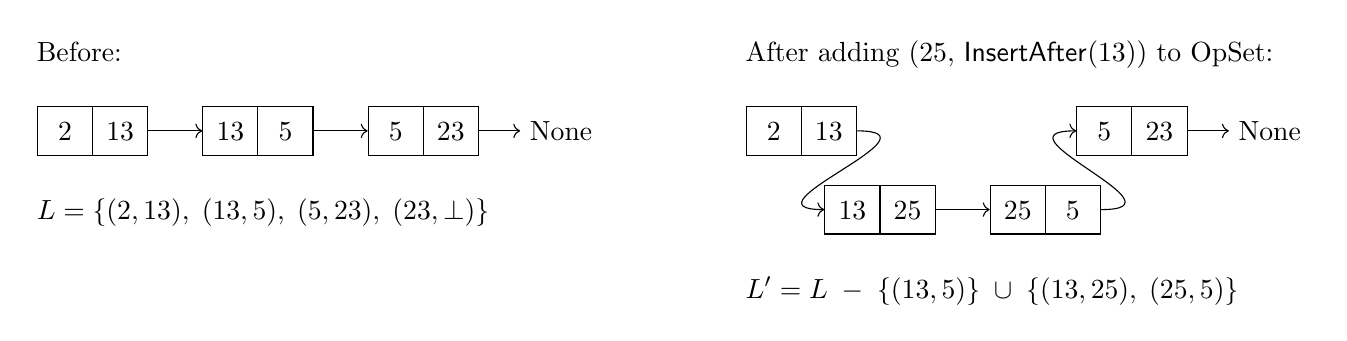
\begin{tikzpicture}
  \tikzstyle{every node}=[anchor=base,minimum width=7mm,text height=9pt,text depth=2pt]
  \node [anchor=west] at (-9,2) {Before:};
  \node [anchor=west] at (-9,0) {$L = \{ (2, 13),\; (13, 5),\; (5, 23),\; (23, \bot) \}$};
  \node [anchor=west] at (0,2) {After adding $(25,\, \mathsf{InsertAfter}(13))$ to OpSet:};
  \node [anchor=west] at (0,-1) {$L' = L \;-\; \{(13, 5)\} \;\cup\; \{(13, 25),\; (25, 5)\}$};
    \matrix [column sep={7mm,between origins},nodes=draw,matrix anchor=west] at (-9,1) {
    \node (l1a) {2};  & \node (l1b) {13}; &&
    \node (l2a) {13}; & \node (l2b) {5};  &&
    \node (l3a) {5};  & \node (l3b) {23}; &&
    \node (l4a) [draw=none] {None}; \\
  };
  \draw [->] (l1b) -- (l2a);
  \draw [->] (l2b) -- (l3a);
  \draw [->] (l3b) -- (l4a);
  \matrix [column sep={7mm,between origins},nodes=draw,matrix anchor=west] at (1,0) {
    \node (n1) {13}; & \node (n2) {25}; &&
    \node (n3) {25}; & \node (n4) {5}; \\
  };
  \matrix [column sep={7mm,between origins},nodes=draw,matrix anchor=west] at (0,1) {
    \node (r1a) {2};  & \node (r1b) {13}; &&&&&
    \node (r3a) {5};  & \node (r3b) {23}; &&
    \node (r4a) [draw=none] {None}; \\
  };
  \draw [->] (r1b.east) .. controls (2.7,1) and (0,0) .. (n1.west);
  \draw [->] (n2) -- (n3);
  \draw [->] (n4.east) .. controls (5.8,0) and (3.2,1) .. (r3a.west);
  \draw [->] (r3b) -- (r4a);
\end{tikzpicture}
\caption{Illustration of the interpretation of an $\mathsf{InsertAfter}$ operation.}\label{fig:list-insert}
\end{figure}

Note that $L$ never shrinks, it only ever grows through interpreting $\mathsf{InsertAfter}$ operations.
When a list element is removed by the function \textsc{removeListIndex} of Listing~\ref{fig:pseudocode}, the effect is that all values are removed from the list element in the element relation $E$, but the list element remains in $L$ as a \emph{tombstone}, so that any concurrent $\mathsf{InsertAfter}$ operations can still locate the referenced list position.

Thus, from a user's point of view a list element only exists if it has at least one associated value in the $E$ relation; any list elements without an associated value should be ignored.
On this basis we can now define the $\mathrm{idxKey}()$ function that is used in Listing~\ref{fig:pseudocode} to translate a list index into a list element ID:
\[ \mathrm{idxKey}_{E,\, L}(\mathit{obj}, \mathit{key}, i) \;=\; \left\{
   \arraycolsep=2pt \def\arraystretch{1.3}
   \begin{array}{llllll}
       \mathrm{idxKey}_{E,\, L}(\mathit{obj}, n, i-1) &
       \quad\text{if }\; i > 0 & \wedge & (\mathit{key}, n) \in L & \wedge &
       \exists\,\mathit{id}, \mathit{val}.\; (\mathit{id}, \mathit{obj}, \mathit{key}, \mathit{val}) \in E \\
       \mathrm{idxKey}_{E,\, L}(\mathit{obj}, n, i) &
       \quad\text{if }\; && (\mathit{key}, n) \in L & \wedge &
       \nexists\,\mathit{id}, \mathit{val}.\; (\mathit{id}, \mathit{obj}, \mathit{key}, \mathit{val}) \in E \\
       \mathit{key} &
       \quad\text{if }\; i = 0 & \wedge &&&
       \exists\,\mathit{id}, \mathit{val}.\; (\mathit{id}, \mathit{obj}, \mathit{key}, \mathit{val}) \in E \\
   \end{array} \right. \]
$\mathit{key}$ is initially the ID of the $\mathsf{MakeList}$ operation that created the list.
The function recursively moves along the linked list structure in $L$, decrementing the index for every list element that has an associated value, and not counting any list elements without associated value (which are treated as deleted).
Eventually, it returns the ID of the list element with the desired index.

\section{Discussion: Merging Text Edits}\label{sec:bad-merge}

The datatypes we have specified in \S~\ref{sec:datatypes} can support a wide range of applications.
For example, the list datatype can be used to implement a collaborative text editor: by treating the text as a list of individual characters, every edit can be expressed as a sequence of insertion or deletion operations on the list.

The problem of collaborative text editing has been studied extensively, using two main approaches: Operational Transformation and CRDTs.
We discuss this prior work in \S~\ref{sec:relwork}.
We will now highlight a scenario that, to our knowledge, has not been considered by any previous work on collaborative text editing.

Consider the execution illustrated in Figure~\ref{fig:bad-merge}.
In this example, two users are concurrently editing a text document that initially reads ``Hello!''.
The user on the left changes it to read ``Hello Alice!'', while concurrently the user on the right changes the document to read ``Hello Charlie!''.
When the concurrent edits are merged, the algorithm randomly interleaves the two insertions of ``~Alice'' and ``~Charlie'' character by character, resulting in an unreadable jumble of characters.

\begin{figure}
\centering
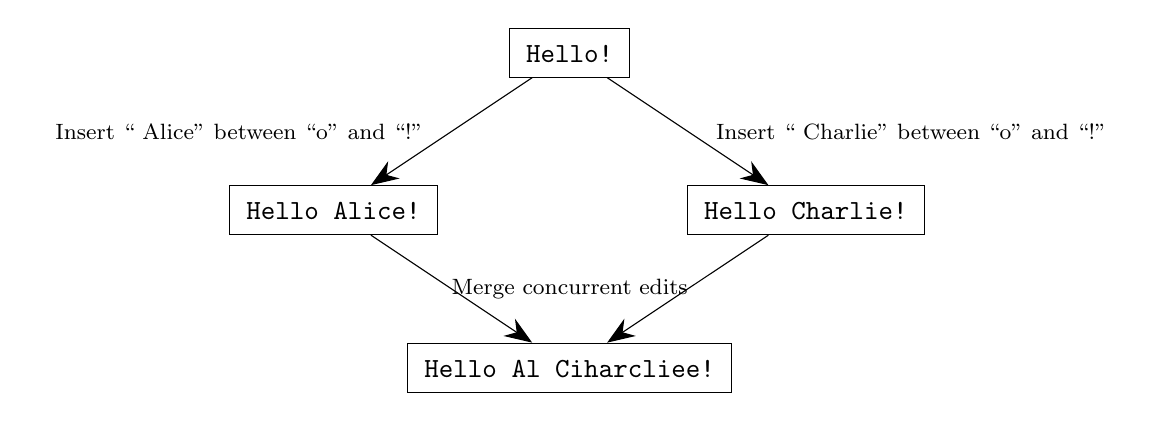
\begin{tikzpicture}
  \tikzstyle{box}=[rectangle,draw,inner xsep=6pt,text height=9pt,text depth=2pt]
  \tikzstyle{every path}=[draw,-{Stealth[length=3.5mm]}]
  \node [box] (start) at (3,4) {\texttt{Hello!}};
  \node [box] (left)  at (0,2) {\texttt{Hello Alice!}};
  \node [box] (right) at (6,2) {\texttt{Hello Charlie!}};
  \node [box] (merge) at (3,0) {\texttt{Hello Al Ciharcliee!}};
  \draw (start) to node [left,inner xsep=10pt,font=\footnotesize]  {Insert ``~Alice'' between ``o'' and ``!''} (left);
  \draw (start) to node [right,inner xsep=10pt,font=\footnotesize] {Insert ``~Charlie'' between ``o'' and ``!''} (right);
  \draw (left)  -- (merge);
  \draw (right) -- (merge);
  \node [text width=3cm,text badly centered,font=\footnotesize] at (3,1) {Merge concurrent edits};
\end{tikzpicture}
\caption{Two concurrent insertions at the same position are interleaved.}\label{fig:bad-merge}
\end{figure}

The problem is even worse if the concurrent insertions are not just a single word, but an entire paragraph or section.
In these cases, interleaving the users' insertions would most likely result in an entirely incomprehensible text that would have to be deleted and rewritten.
Even though the merge in Figure~\ref{fig:bad-merge} is so obviously undesirable, there is to our knowledge no formal specification of collaborative text editing that rules out such an interleaving of insertions.

\begin{theorem}\label{thm:attiya-allows-interleaving}
    The $\mathcal{A}_\textsf{strong}$ specification of collaborative text editing by Attiya et al. \cite{Attiya:2016kh} allows the outcome in Figure~\ref{fig:bad-merge}; that is, an algorithm that interleaves concurrent insertions at the same position may nevertheless satisfy the $\mathcal{A}_\textsf{strong}$ specification.
    Moreover, the text editing CRDT algorithms Logoot \cite{Weiss:2009ht,Weiss:2010hx} and LSEQ \cite{Nedelec:2016eo,Nedelec:2013ky} also allow this outcome.
\end{theorem}
\begin{proof}
    Follows directly from the respective definitions, which are all based on the idea of assigning each character a position in a totally ordered identifier space, such that the order of identifiers corresponds to the order of characters in the document.
    When a new character is inserted, it is assigned an identifier that lies somewhere between the identifiers of its predecessor and successor.
    However, when concurrent insertions with the same predecessor and successor are performed, those insertions are ordered arbitrarily.
    Repeated insertions within the same predecessor-successor interval may thus be interleaved arbitrarily.

    We also performed tests with open source implementations of Logoot \cite{AhmedNacer:2011ke,ReplicationBenchmark} and LSEQ \cite{LSEQTree,Nedelec:2016eo}, and observed this interleaving anomaly occurring in practice.
\end{proof}

Rather than interleaving characters, a better approach to merging is to keep all insertions by a particular user together as a continuous sequence.
With this constraint, there are two acceptable merged results in the example of Figure~\ref{fig:bad-merge}: either ``Hello Alice Charlie!'' or ``Hello Charlie Alice!''.
The choice between these two outcomes is arbitrary, as there is no \emph{a priori} requirement for one user's insertions to come before the other's.

\begin{theorem}\label{thm:no-interleaving}
    The list specification from \S~\ref{sec:datatypes} does not allow interleaving of concurrent insertions.
    That is, if one user inserts a character sequence $\langle x_1, x_2, \dots, x_n \rangle$ and another user concurrently inserts a character sequence $\langle y_1, y_2, \dots, y_m \rangle$ at the same position, the merged document contains either the character sequence $\langle x_1, x_2, \dots, x_n, y_1, y_2, \dots, y_m \rangle$ or the character sequence $\langle y_1, y_2, \dots, y_m, x_1, x_2, \dots, x_n \rangle$ at the specified position.
\end{theorem}
\begin{proof}
    We formalise the list specification and Theorem~\ref{thm:no-interleaving} using the Isabelle/HOL proof assistant~\cite{DBLP:conf/tphol/WenzelPN08}.
    \ifarxiv
        The formal proof development is summarised in Appendix~\ref{appendix:no-interleaving}.
    \else
        For space reasons, we elide the formal proof development; it is described in the extended version of this paper \cite{ExtendedVersion,AFP}.
    \fi
\end{proof}

For an informal argument why interleaving is ruled out, see Figure~\ref{fig:op-permutations}, which shows an editing scenario similar to Figure~\ref{fig:bad-merge}, but with the insertions of ``~Alice'' and ``~Charlie'' shortened to ``Al'' and ``Ch'' respectively.
The example contains four insertion operations (``A'', ``l'', ``C'', and ``h''), which can be ordered in six possible ways.
However, among the six possible operation orderings there are only two possible results: \texttt{ChAl} or \texttt{AlCh}.
Interleavings such as \texttt{CAhl} or \texttt{AChl} never occur.

In fact, the end result depends only on the relative ordering of the operations that insert ``A'' and ``C'', respectively.
All other operations can be reordered without affecting the outcome.
Thus, even if the inserted strings are longer than two characters, their relative ordering only depends on the IDs of their first character.
The remaining characters follow their initial character without interleaving.

Note that there are only six possible orderings of the four operations, and not $4! = 24$, because the Lamport timestamp ordering on identifiers (as given in \S~\ref{sec:system-model}) is a linear extension of the causal order.
In this example we assume that text is typed from left to right (that is, ``A'' is always inserted before ``l'', and ``C'' is inserted before ``h'').
This implies that the ID of the operation inserting ``l'' must be greater than that of the insertion of ``A'', and likewise the ``h'' insertion must be greater than the ``C'' insertion.

\begin{figure}
% ``A'', ``l'', ``C'', ``h''
% ``A'', ``C'', ``l'', ``h''
% ``A'', ``C'', ``h'', ``l''
% ``C'', ``A'', ``l'', ``h''
% ``C'', ``A'', ``h'', ``l''
% ``C'', ``h'', ``A'', ``l''
\setlength{\tabcolsep}{1pt}
\begin{tabular}{ll|ll|ll}
$\mathit{id}_1, \mathsf{InsertAfter}(\mathit{id}_0), \text{``A''}$ & $\rightarrow$ \texttt{A} &
$\mathit{id}_1, \mathsf{InsertAfter}(\mathit{id}_0), \text{``A''}$ & $\rightarrow$ \texttt{A} &
$\mathit{id}_1, \mathsf{InsertAfter}(\mathit{id}_0), \text{``A''}$ & $\rightarrow$ \texttt{A} \\
%%%%%%%%%%
$\mathit{id}_2, \mathsf{InsertAfter}(\mathit{id}_1), \text{``l''}$ & $\rightarrow$ \texttt{Al} &
$\mathit{id}_2, \mathsf{InsertAfter}(\mathit{id}_0), \text{``C''}$ & $\rightarrow$ \texttt{CA} &
$\mathit{id}_2, \mathsf{InsertAfter}(\mathit{id}_0), \text{``C''}$ & $\rightarrow$ \texttt{CA} \\
%%%%%%%%%%
$\mathit{id}_3, \mathsf{InsertAfter}(\mathit{id}_0), \text{``C''}$ & $\rightarrow$ \texttt{CAl} &
$\mathit{id}_3, \mathsf{InsertAfter}(\mathit{id}_1), \text{``l''}$ & $\rightarrow$ \texttt{CAl} &
$\mathit{id}_3, \mathsf{InsertAfter}(\mathit{id}_2), \text{``h''}$ & $\rightarrow$ \texttt{ChA} \\
%%%%%%%%%%
$\mathit{id}_4, \mathsf{InsertAfter}(\mathit{id}_3), \text{``h''}$ & $\rightarrow$ \texttt{ChAl} &
$\mathit{id}_4, \mathsf{InsertAfter}(\mathit{id}_2), \text{``h''}$ & $\rightarrow$ \texttt{ChAl} &
$\mathit{id}_4, \mathsf{InsertAfter}(\mathit{id}_1), \text{``l''}$ & $\rightarrow$ \texttt{ChAl} \\[6pt] \hline &&&&&\\[-6pt]
%%%%%%%%%%
$\mathit{id}_1, \mathsf{InsertAfter}(\mathit{id}_0), \text{``C''}$ & $\rightarrow$ \texttt{C} &
$\mathit{id}_1, \mathsf{InsertAfter}(\mathit{id}_0), \text{``C''}$ & $\rightarrow$ \texttt{C} &
$\mathit{id}_1, \mathsf{InsertAfter}(\mathit{id}_0), \text{``C''}$ & $\rightarrow$ \texttt{C} \\
%%%%%%%%%%
$\mathit{id}_2, \mathsf{InsertAfter}(\mathit{id}_0), \text{``A''}$ & $\rightarrow$ \texttt{AC} &
$\mathit{id}_2, \mathsf{InsertAfter}(\mathit{id}_0), \text{``A''}$ & $\rightarrow$ \texttt{AC} &
$\mathit{id}_2, \mathsf{InsertAfter}(\mathit{id}_1), \text{``h''}$ & $\rightarrow$ \texttt{Ch} \\
%%%%%%%%%%
$\mathit{id}_3, \mathsf{InsertAfter}(\mathit{id}_2), \text{``l''}$ & $\rightarrow$ \texttt{AlC} &
$\mathit{id}_3, \mathsf{InsertAfter}(\mathit{id}_1), \text{``h''}$ & $\rightarrow$ \texttt{ACh} &
$\mathit{id}_3, \mathsf{InsertAfter}(\mathit{id}_0), \text{``A''}$ & $\rightarrow$ \texttt{ACh} \\
%%%%%%%%%%
$\mathit{id}_4, \mathsf{InsertAfter}(\mathit{id}_1), \text{``h''}$ & $\rightarrow$ \texttt{AlCh} &
$\mathit{id}_4, \mathsf{InsertAfter}(\mathit{id}_2), \text{``l''}$ & $\rightarrow$ \texttt{AlCh} &
$\mathit{id}_4, \mathsf{InsertAfter}(\mathit{id}_3), \text{``l''}$ & $\rightarrow$ \texttt{AlCh} \\
\end{tabular}
\caption{All possible operation orderings when the strings ``Al'' (for ``Alice'') and ``Ch'' (for ``Charlie'') are concurrently inserted at the same position.
The operation IDs are arbitrary; we only require that $id_0 < id_1 < id_2 < id_3 < id_4$.}\label{fig:op-permutations}
\end{figure}

\begin{theorem}
    The OpSet list specification from \S~\ref{sec:datatypes} is strictly stronger than the $\mathcal{A}_\textsf{strong}$ specification of Attiya et al \cite{Attiya:2016kh}.
    That is, any algorithm that satisfies the list specification given in \S~\ref{sec:datatypes} also satisfies $\mathcal{A}_\textsf{strong}$, but the converse is not true.
\end{theorem}
\begin{proof}
    We formalise the $\mathcal{A}_\textsf{strong}$ specification with Isabelle/HOL, and produce a mechanically verified proof that every possible execution of the list specification from \S~\ref{sec:datatypes} satisfies all conditions of $\mathcal{A}_\textsf{strong}$.
    \ifarxiv
        The formal proof development is summarised in Appendix~\ref{appendix:attiya-spec}.
    \else
        The formal proof development is described in the extended version of this paper \cite{ExtendedVersion,AFP}.
    \fi
    The fact that our specification is \emph{strictly} stronger follows from Theorems~\ref{thm:attiya-allows-interleaving} and~\ref{thm:no-interleaving}.
\end{proof}

\begin{theorem}
    The RGA algorithm \cite{Roh:2011dw} satisfies the OpSet list specification introduced in this paper, while Logoot \cite{Weiss:2009ht,Weiss:2010hx} and LSEQ \cite{Nedelec:2016eo,Nedelec:2013ky} do not.
\end{theorem}
\begin{proof}
    We use Isabelle/HOL to prove that RGA satisfies our specification, as described in
    \ifarxiv
        Appendix~\ref{appendix:rga}.
    \else
        the extended version of this paper \cite{ExtendedVersion,AFP}.
    \fi
    Our Isabelle/HOL implementation of RGA is based on the formalisation that we developed in previous work \cite{Gomes:2017vo,Gomes:2017gy}.
    The fact that Logoot and LSEQ do not satisfy our specification follows directly from Theorems~\ref{thm:attiya-allows-interleaving} and~\ref{thm:no-interleaving}.
\end{proof}

\section{Specifying a Tree Datatype}\label{sec:tree}

Tree data structures are useful in many applications: for example, file systems (consisting of directories and files) and XML or JSON documents are trees.
In this section we build upon the data structures of \S~\ref{sec:datatypes} to specify a collaboratively editable tree datatype.
Branch nodes in this tree may be either maps or lists, and leaf nodes are primitive values (wrapped in a $\mathsf{MakeVal}$ operation).

Unlike previous CRDTs for tree data structures \cite{Martin:2010ih,Kleppmann:2016ve}, our datatype supports an \emph{atomic move} operation, which can move an entire subtree to a new location, or rename a key in a map, or reorder items in a list.
Moving an item is not the same as deleting it and re-inserting it in a new location: if two users concurrently delete and re-insert the same item, it would be duplicated.
On the other hand, if two users concurrently move the same item to different locations, the move operation with the greater ID will determine the item's final location.

A tree is a restricted form of the object graph specified in \S~\ref{sec:datatypes}.
First, we require that there is a designated root object: assume that we have an operation ID $\mathsf{root}$ that is less than all other operation IDs (according to the total order on identifiers, introduced in \S~\ref{sec:system-model}).
Further assume that for any OpSet $O$ specifying a tree, we have either $(\mathsf{root},\, \mathsf{MakeList}) \in O$ or $(\mathsf{root},\, \mathsf{MakeMap}) \in O$, depending on whether the root node is a list or a map.
We define an object $x$ to be the \emph{parent} of an object $y$ if one of the values in $x$ is a reference to $y$.
The \emph{ancestor} relation is the transitive closure of the parent relation, defined using the element relation $E$:
\begin{align*}
    \mathrm{parent}(E,\, i) &=
    \begin{cases}
        \big\{ (\mathit{obj}, \mathit{val}) \mid \exists\,\mathit{id}, \mathit{key}.\;
            (\mathit{id}, \mathit{obj}, \mathit{key}, \mathit{val}) \in E \big\} & \text{if } i=1 \\
        \big\{ (x, z) \mid (x, y) \in \mathrm{parent}(E,\, i-1) \;\wedge\;
            (y, z) \in \mathrm{parent}(E,\, 1) \big\} & \text{if } i > 1
    \end{cases} \\[8pt]
    \mathrm{ancestor}(E) &= \bigcup_{i \;\geq\; 1} \mathrm{parent}(E,\, i)
\end{align*}

An object graph is a tree if the root has no parent, every non-root node has exactly one parent, and if the ancestor relation has no cycles.
We can redefine the operation interpretations from \S~\ref{sec:datatypes-interp} to preserve this tree invariant.
In fact, it is sufficient to redefine the interpretation of $\mathsf{Assign}$, and leave the interpretation of the other five operation types unchanged:
\begin{align*}
    \mathrm{interp}&\big[(E,\, L),\; (\mathit{id},\, \mathsf{Assign}(\mathit{obj}, \mathit{key}, \mathit{val}, \mathit{prev})) \big] \;=\\
    & \left\{
    \arraycolsep=0pt \def\arraystretch{1.5}
    \begin{array}{l}
        (E,\, L) \qquad \text{if } (\mathit{val},\, \mathit{obj}) \in \mathrm{ancestor}(E) \\[2pt]
        \Big( \big\{ (\mathit{id}', \mathit{obj}', \mathit{key}', \mathit{val}') \in E \mid
        \mathit{id}' \notin \mathit{prev} \wedge \mathit{val}' \neq \mathit{val} \big\} \;\cup\;
        \big\{ (\mathit{id}, \mathit{obj}, \mathit{key}, \mathit{val}) \big\},\; L \Big) \\
        \hphantom{(E,\, L)} \qquad \text{if } (\mathit{val},\, \mathit{obj}) \notin \mathrm{ancestor}(E)
    \end{array} \right.
\end{align*}

This definition differs in two ways from that in \S~\ref{sec:datatypes-interp}.
Firstly, the operation has no effect if the value $\mathit{val}$ is already an ancestor of the proposed parent $\mathit{obj}$, since the operation would otherwise introduce a cycle.
Secondly, any existing tuple in $E$ that references the same value $\mathit{val}$ is removed, preserving the invariant that every non-root node must have exactly one parent.

Intuitively, this interpretation of $\mathsf{Assign}$ performs an atomic move whenever $\mathit{val}$ is the ID of an existing object in the tree; in that case, it is moved from its existing position to the key $\mathit{key}$ in the object $\mathit{obj}$.
If $\mathit{val}$ does not currently exist in the tree (e.g.\ because it has just been created), the operation behaves like conventional assignment.

\subsection{Discussion: Subtree Move Conflicts}

In a replicated tree datatype with move operations, concurrent moves may conflict in various ways \cite{Najafzadeh:2017vk,AhmedNacer:2012us,Tao:2015gd}.
For example, two different operations may concurrently move the same object to different positions; we resolve this conflict by letting the operation with the greatest identifier ``win''.
Intuitively, we can think of the location of an object in the tree as being determined by a last-writer-wins register, and a move operation overwrites that register.

\begin{figure}
\centering
\begin{tikzpicture}
  \tikzstyle{arrow}=[draw,-{Stealth[length=3.5mm]}]
  \node [rectangle,draw] (start) at (4,4) {
      \begin{tikzpicture}
      \node {$\mathsf{root}$} [level distance=9mm] child {node {$a$}} child {node {$b$}};
      \end{tikzpicture}
  };
  \node [rectangle,draw] (left) at (1,2) {
      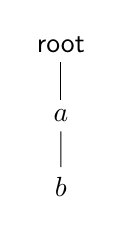
\begin{tikzpicture}
      \node {$\mathsf{root}$} [level distance=9mm] child {node {$a$} child {node {$b$}}};
      \end{tikzpicture}
  };
  \node [rectangle,draw] (right) at (7,2) {
      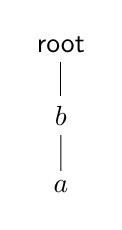
\begin{tikzpicture}
      \node {$\mathsf{root}$} [level distance=9mm] child {node {$b$} child {node {$a$}}};
      \end{tikzpicture}
  };
  \node [rectangle,draw] (merge) at (4,0) { ? };
  \node at (0,4) {$(\mathit{id}_1,\, \mathsf{Assign}(a,\, \mathit{key}_1,\, b,\, \emptyset))$};
  \node at (8,4) {$(\mathit{id}_2,\, \mathsf{Assign}(b,\, \mathit{key}_2,\, a,\, \emptyset))$};
  \draw [arrow] (start.west) -- (left);
  \draw [arrow] (start.east) -- (right);
  \draw [arrow] (left)  -- (merge.north west);
  \draw [arrow] (right) -- (merge.north east);
  \node at (4,1) {merge};
\end{tikzpicture}
\caption{Initially, $a$ and $b$ are siblings. On one node, $b$ is moved to be a child of $a$, while concurrently on another node,
$a$ is moved to be a child of $b$. What should the final outcome be?}\label{fig:concurrent-move}
\end{figure}

A more subtle kind of conflict is illustrated in Figure~\ref{fig:concurrent-move}.
Here, two different objects $a$ and $b$, which are originally siblings, are concurrently moved to be children of each other.
If the move semantics are not defined carefully, it could happen that $a$ and $b$ form a cycle, violating the tree invariant.
Our interpretation function for $\mathsf{Assign}$ handles this situation based on the ordering of the operation IDs $\mathit{id}_1$ and $\mathit{id}_2$.
Since operations are interpreted in order of ascending identifier, one of the two (say, $\mathit{id}_1$) is interpreted first.
When the second ($\mathit{id}_2$) is subsequently interpreted, $a$ is already an ancestor of $b$, and thus the second operation has no effect.

On some nodes, operation $\mathit{id}_2$ may be applied first, and $\mathit{id}_1$ applied later.
In this case, the user will first observe $b$ becoming a child of $a$, and later observe their positions being swapped (with the effect of $\mathit{id}_2$ being undone).

\section{Related Work}\label{sec:relwork}

Algorithms for collaboratively editing a shared data structure have been the topic of active research for approximately 30 years, under the headings of Operational Transformation \cite{Ellis:1989ue,Nichols:1995fd,Ressel:1996wx,Sun:1998un,Sun:1998vf,Suleiman:1997gl,Suleiman:1998eu,Vidot:2000ch,Imine:2003ks,Li:2004er,Li:2008hw,Oster:2006tr} and CRDTs \cite{Shapiro:2011wy,Shapiro:2011un,Roh:2011dw,Preguica:2009fz,Oster:2006wj,Weiss:2010hx,Nedelec:2013ky,Nedelec:2016eo,Grishchenko:2014eh,Kleppmann:2016ve}.

However, throughout this time, the exact consistency properties provided by the algorithms have been somewhat unclear.
For example, Sun et al.~\cite{Sun:1998un} identified three desirable properties that they articulated informally: \emph{convergence}, \emph{causality preservation}, and \emph{intention preservation}.
While the definition of the first two properties is fairly unambiguous, the definition of ``intention preservation'' leaves much more room for interpretation.
Sun et al.\ define it as follows \cite{Sun:1998un}:
\begin{displayquote}
For any operation $O$, the effects of executing $O$ at all sites are the same as the intention of $O$, and the effect of executing $O$ does not change the effects of independent operations.
\end{displayquote}
where the term \emph{intention} is in turn defined as:
\begin{displayquote}
The intention of an operation $O$ is the execution effect which can be achieved by applying $O$ on the document state from which $O$ was generated.
\end{displayquote}
Efforts to formally specify and verify the semantics of replicated datatypes have replaced informal statements of this type with more precise definitions of consistency properties.

\subsection{Specification and Verification}

Bieniusa et al.~\cite{Bieniusa:2012gt} articulate a \emph{principle of permutation equivalence} that partially specifies the expected semantics of replicated datatypes, but which leaves some combinations of operations unspecified.
Burckhardt et al.~\cite{Burckhardt:2014ft} give a complete specification of CRDT counters, registers, and sets, and show how to verify that algorithms satisfy these specifications in hand-written proofs.
Zeller et al.~\cite{Zeller:2014fl} formalise the same datatypes using Isabelle/HOL and provide mechanised proofs of their correctness.
These papers do not consider lists, maps, or tree datatypes.

Gomes et al.~\cite{Gomes:2017gy} establish a formal verification framework for CRDTs in Isabelle/HOL, and verify the strong eventual consistency properties (in particular, convergence) of a list, set, and counter datatype.
However, the work does not specify the datatype semantics beyond the convergence property.

Attiya et al.~\cite{Attiya:2016kh} give two specifications of collaborative text editing ($\mathcal{A}_\textsf{strong}$ and $\mathcal{A}_\textsf{weak}$), prove that the RGA CRDT \cite{Roh:2011dw} satisfies $\mathcal{A}_\textsf{strong}$, and conjecture that the Operational Transformation algorithm Jupiter \cite{Nichols:1995fd} satisfies $\mathcal{A}_\textsf{weak}$.
Wei et al.~\cite{Wei:2017tg} complete the proof that Jupiter satisfies $\mathcal{A}_\textsf{weak}$.

XXX: also~\cite{DBLP:conf/popl/BurckhardtGYZ14, DBLP:conf/atva/MukundRS15, DBLP:conf/coordination/GadducciMR17, DBLP:conf/popl/GotsmanYFNS16}

\subsection{Collaborative Tree Datatypes}

For collaborative editing of tree data structures, several CRDTs \cite{Martin:2010ih,Kleppmann:2016ve} and Operational Transformation algorithms \cite{Jungnickel:2016cb,Ignat:2003jy,Davis:2002iv} have been proposed.
However, most of them only consider insertion and deletion of tree nodes, but do not support a move operation.

As explained in Section~\ref{sec:tree}, supporting an operation that can move a subtree to a new location within a tree raises the possibility of some particular conflicts that need to be handled.
Ahmed-Nacer et al.~\cite{AhmedNacer:2012us} survey approaches to handling these conflicts without providing concrete algorithms.
Tao et al.~\cite{Tao:2015gd} propose handling conflicting move operations by allowing the same object to appear in more than one location; thus, their datatype is strictly a DAG, not a tree.

Najafzadeh~\cite{Najafzadeh:2017vk} asserts that concurrent move operations on a tree cannot safely be implemented in a CRDT, since the precondition of a move operation is not stable.
The proposed solution in this work is to use locks to globally synchronise move operations, thus preventing a scenario such as that in Figure~\ref{fig:concurrent-move} from ever occurring.
However, the resulting datatype is not strictly a CRDT, since some operations require strongly consistent synchronisation.

To our knowledge, our move semantics specified in Section~\ref{sec:tree} is the first definition of such an operation on a fully asynchronous tree CRDT.
We avoid the apparent contradiction with Najafzadeh's assertion by evaluating the precondition $(\mathit{val},\, \mathit{obj}) \notin \mathrm{ancestor}(E)$ at the same time as applying the operation, rather than at the time when the operation is generated, and by applying all operations in the OpSet in a deterministic order.

\subsection{Ordered Sets of Operations}

Baquero et al.~\cite{Baquero:2014ed} and Grishchenko~\cite{Grishchenko:2014eh} have previously proposed representing CRDTs in terms of a partially-ordered log of operations (where the partial order captures the causal relationships between operations).
Our OpSet is a straightforward variant of this idea, in which we define the total order on identifiers to be a linear extension of the partial order that captures causality.
This linear extension is well-known and goes back to Lamport~\cite{Lamport:1978jq}.

Our approach of sequentially interpreting operations, in order of $\mathit{id}$, is reminiscent of the concept of \emph{serializability} in databases: the data structure obtained by interpreting an OpSet is equal to the outcome of applying the operations in their serial order, even if the execution that produced the OpSet was in fact concurrent.
However, conventional transaction serializability requires synchronous coordination between replicas \cite{Davidson:1985hv}.
We circumvent this limitation, and hence allow nodes to make progress while offline, by allowing the interpretation of an operation to change if another operation with a lower ID is delivered.


\section{Conclusion}

In this work we have introduced Operation Sets (OpSets), a simple but expressive approach for specifying the semantics of replicated datatypes.
We specified a variety of common, composable replicated datatypes in the OpSets model, and used Isabelle/HOL to formally reason about their properties.
We have also shown how the OpSet abstraction can be used to reason about existing replication algorithms, and developed a new specification to highlighted an interleaving anomaly that affects some existing collaborative text editing algorithms.
Finally we demonstrated how the OpSet model to can be used to develop new specifications to support algorithm design, and developed a specification for an atomic move operation in a tree CRDT.

The OpSets approach is a form of executable specification that precisely defines the permitted states of a replica after some set of updates have been applied.
The simplicity of our approach builds on sequential OpSet interpretation: operations are applied in strict ascending order of ID.
This property is very useful as it simplifies reasoning when writing new specifications and allows CRDT designers to quickly write new specifications or invariants for CRDTs.
This contrasts with the traditional approach, where analysis or design must deal with the complexities of concurrent modification and allow operations to be applied in any causal order due to commutativity.
We took advantage of the ease of specification to demonstrate the correspondence between sequential specification and commutative implementation, proving that the RGA CRDT satisfies our OpSet specification of lists.
For future work it will be interesting to further explore this correspondence for other datatypes; in particular, we hypothesise that it is possible to derive a tree CRDT with a commutative move operation from the specification in \S~\ref{sec:tree}.

%More generally, one can regard the OpSet as a \emph{database of facts}, containing all changes ever made to the shared data, and the interpretation function a \emph{query} over this database, with the resulting datatype being a \emph{materialized view} in database terminology.
%When new operations are added to an OpSet $O$, computing the corresponding change to $\llbracket O \rrbracket$ is a \emph{materialized view maintenance} problem, which has been studied extensively in the database literature \cite{Gupta:1999uz}.
%We have found that thinking about replicated datatypes as materialized views onto an OpSet a useful perspective for understanding and improving replication algorithms, and in future work we aim to explore this idea more fully.

\subsection*{Acknowledgements}

The authors wish to acknowledge the support of The Boeing Company,
the EPSRC ``REMS: Rigorous Engineering for Mainstream Systems'' programme grant (EP/K008528), and
the EPSRC ``Interdisciplinary Centre for Finding, Understanding and Countering Crime in the Cloud'' grant (EP/M020320).
We thank KC Sivaramakrishnan and Peter Sewell for their helpful feedback on this paper.

\newpage

\bibliographystyle{plainnat}
\bibliography{references}{}

\newpage

\appendix

\section{Introduction to Isabelle/HOL}
\label{sect:appendix:isabelle}

% cribbed from oopsla paper with some small changes and deletions
% TODO: further edit down as required

We provide a brief introduction to the key concepts and syntax of Isabelle/HOL so that the unfamiliar reader can understand the material in Appendix~\ref{sect:appendix:statements}.
A more detailed introduction can be found in the standard tutorial material~\cite{DBLP:books/sp/NipkowK14}.

\paragraph{Syntax of expressions.}

Isabelle/HOL is a logic with a strict, polymorphic, inferred type system.
\emph{Function types} are written $\tau_1 \Rightarrow \tau_2$, and are inhabited by \emph{total} functions, mapping elements of $\tau_1$ to elements of $\tau_2$.
We write $\tau_1 \times \tau_2$ for the \emph{product type} of $\tau_1$ and $\tau_2$, inhabited by pairs of elements of type $\tau_1$ and $\tau_2$, respectively.
In a similar fashion to Standard ML and OCaml, \emph{type operators} are applied to arguments in reverse order, and therefore $\tau\ \isa{list}$ denotes the type of lists of elements of type $\tau$, and $\tau\ \isa{set}$ denotes the type of mathematical (i.e., potentially infinite) sets of type $\tau$.
Type variables are written in lowercase, and preceded with a prime: ${\isacharprime}a \Rightarrow {\isacharprime}a$ denotes the type of a polymorphic identity function, for example.
\emph{Tagged union} types are introduced with the $\isacommand{datatype}$ keyword, with constructors of these types usually written with an initial upper case letter.

In Isabelle/HOL's term language we write $\isa{t} \mathbin{::} \tau$ for a \emph{type ascription}, constraining the type of the term $\isa{t}$ to the type $\tau$.
We write $\lambda{x}.\: t$ for an anonymous function mapping an argument $\isa{x}$ to $\isa{t(x)}$, and write the application of term $\isa{t}$ with function type to an argument $\isa{u}$ as $\isa{t\ u}$, as usual.
Terms of list type are introduced using one of two constructors: the empty list $[\,]$ or `nil', and the infix operator $\isa{\#}$ which is pronounced ``cons'', and which prepends an element to an existing list.
We use $[t_1, \ldots, t_n]$ as syntactic sugar for a list literal, and $\isa{xs} \mathbin{\isacharat} \isa{ys}$ to express the concatenation (appending) of two lists $\isa{xs}$ and $\isa{ys}$.
We write $\{\,\}$ for the empty set, and use usual mathematical notation for set union, disjunction, membership tests, and so on: $\isa{t} \cup \isa{u}$, $\isa{t} \cap \isa{u}$, and $\isa{x} \in \isa{t}$.
We write $t \longrightarrow s$ for logical implication between formulae (terms of type $\isa{bool}$).
Strictly speaking Isabelle is a logical framework, providing a weak meta-logic within which object logics are embedded, including the Isabelle/HOL object logic that we use in this work.
Accordingly, the implication arrow of Isabelle's meta-logic, $\isa{t} \Longrightarrow \isa{u}$, is required in certain contexts over the object-logic implication arrow, $t \longrightarrow s$, already introduced.
However, for purposes of an intuitive understanding, the two forms of implication can be regarded as equivalent by the reader, with the requirement to use one over the other merely being an implementation detail of Isabelle itself.
We will sometimes use the shorthand ${\isasymlbrakk}\isa{H}_1{\isacharsemicolon}\ \ldots{\isacharsemicolon}\ \isa{H}_n{\isasymrbrakk}\ {\isasymLongrightarrow}\ C$ instead of iterated meta-logic implications, i.e., $H_1\ {\isasymLongrightarrow}\ \ldots\ {\isasymLongrightarrow}\ H_n\ {\isasymLongrightarrow}\ C$.

\paragraph{Definitions and theorems.}

New non-recursive definitions are entered into Isabelle's global context using the $\mathbf{definition}$ keyword.
Recursive functions are defined using the $\mathbf{fun}$ keyword, and support pattern matching on their arguments.
All functions are total, and therefore every recursive function must be provably terminating.
All termination proofs in this work are generated automatically by Isabelle itself.

Inductive relations are defined with the $\mathbf{inductive}$ keyword.
For example, the definition
\begin{isabelle}
\isacommand{inductive} only-fives\ {\isacharcolon}{\isacharcolon}\ {\isachardoublequoteopen}nat\ list\ {\isasymRightarrow}\ bool{\isachardoublequoteclose}\ \isakeyword{where}\\
{\isachardoublequoteopen}only-fives\ {\isacharbrackleft}{\isacharbrackright}{\isachardoublequoteclose}\ {\isacharbar}\\
{\isachardoublequoteopen}{\isasymlbrakk}\ only-fives\ xs\ {\isasymrbrakk}\ {\isasymLongrightarrow}\ only-fives {\isacharparenleft}5\#xs{\isacharparenright}{\isachardoublequoteclose}
\end{isabelle}
\noindent %dpm: spacing above
introduces a new constant $\isa{only-fives}$ of type $\isa{nat list} \Rightarrow \isa{bool}$.
The two clauses in the body of the definition enumerate the conditions under which $\isa{only-fives}\ \isa{xs}$ is true, for arbitrary $\isa{xs}$: firstly, $\isa{only-fives}$ is true for the empty list; and secondly, if you know that $\isa{only-fives}\ \isa{xs}$ is true for some $\isa{xs}$, then you can deduce that $\isa{only-fives}\ (5\#\isa{xs})$ (i.e., $\isa{xs}$ prefixed with the number 5) is also true.
Moreover, $\isa{only-fives}\ \isa{xs}$ is true in no other circumstances---it is the \emph{smallest} relation closed under the rules defining it.
In short, the clauses above state that $\isa{only-fives}\ \isa{xs}$ holds exactly in the case where $\isa{xs}$ is a (potentially empty) list containing only repeated copies of the natural number $5$.

Lemmas, theorems, and corollaries can be asserted using the $\isacommand{lemma}$, $\isacommand{theorem}$, and $\isacommand{corollary}$ keywords, respectively.
There is no semantic difference between these keywords in Isabelle.
For example,
\begin{isabelle}
\isacommand{theorem} only-fives-concat{\isacharcolon}\\
\isakeyword{assumes}\ only-fives\ xs \isakeyword{and}\ only-fives\ ys\\
\isakeyword{shows}\ only-fives\ (xs \isacharat ys)
\end{isabelle}
\noindent %dpm: spacing above
conjectures that if $\isa{xs}$ and $\isa{ys}$ are both lists of fives, then their concatenation $xs \mathbin{\isacharat} ys$ is also a list of fives.
Isabelle then requires that this claim be proved by using one of its proof methods, for example by induction.
Some proofs can be automated, whilst others require the user to provide explicit reasoning steps.
The theorem is assigned a name, here $\isa{only-fives-concat}$, so that it may be referenced in later proofs.

\newpage

\section{Statements of Mechanised Proofs}
\label{sect:appendix:statements}

\end{document}
